\appendices
\section{Discretization Error}\label{app:discretization-correction-proof}
\begin{restatable}{theorem}{discretizationthm}

\label{thm:discretization-correction}
	Consider any interval $[\nn(j_1), \nn(j_2)]$ for $ 0 \leq j_1 < j_2 \leq j_{\max}$ and let $e_{j_1, j_2}$ denote the error between
	$\psi$ and $\psihat$ over all the discretization points in the interval $[\nn(j_1), \nn(j_2)]$. Also, let $c_{\max}$ be the
	maximum absolute value of the slope of any piece of $\psihat$ over the interval
	\begin{equation*}
	    e_{j_1, j_2} \leq \max_{z \in [\nn(j_1), \nn(j_2)]} | \psi(z) - \psihat(z) | \leq e_{j_1, j_2} + (c_{\max} + \psi'_{\max}) \Delta\,
	\end{equation*}
	wherein $\psi'_{\max} = \max_{z \in [\nn(j_1), \nn(j_2)]} \left| \frac{d \psi}{dz} \right| $.
\end{restatable}
We start by proving a useful lemma that derives an error bound for an interval between two consecutive grid points $[\nn(j), \nn(j+1)]$ for $1 \leq j < j_{\max}$.
\begin{lemma}\label{Lemma:useful-lemma-1}
    Let $e_j = | \psi(\nn(j)) - \psihat(\nn(j)) |$ for some index $j \in [1, j_{\max})$. For any $z \in [\nn(j), \nn(j+1)]$, the error $ | \psi(z) - \psihat(z) | \leq e_j + \left( \psi'_{\max} + |c| \right) \Delta $, wherein $\psi'_{\max} = \max_{z \in [\nn(j), \nn(j+1))} \left| \frac{d \psi}{dz} \right|$ and $ \psihat(z) = c z + d$ for $z \in  [\nn(j), \nn(j+1)]$
\end{lemma}
\begin{proof}
    Consider any $z \in [\nn(j), \nn(j+1)]$. Note that by the mean value theorem: $\psi(z) = \psi(\nn(j)) + \psi'(z^*) (z - \nn(j))$ for some $z^* \in [\nn(j), z]$. Therefore, we have, $ | \psi(z) - \psi(\nn(j))| \leq | \psi'(z^*)| \times  | z - \nn(j)| \leq \psi'_{\max} \Delta$ which leads us to:
    \begin{align*}
        | \psi(z) - \psihat(z) | 
            & \leq | \psi(z) - \psi(\nn(j)) + \psi(\nn(j) - \psihat(\nn(j)) + \psihat(\nn(j)) - \psihat(z) | \\
		& \leq | \psi(z) - \psi(\nn(j)) | + | \psi(\nn(j) - \psihat(\nn(j)) | + |  \psihat(\nn(j)) - \psihat(z) | \\
            & \leq \psi'_{\max} \Delta + e_j + | c (z - \nn(j)) |\;\; \leq \;\; e_j + \left( \psi'_{\max} + |c| \right) \Delta \qedhere
	\end{align*}
\end{proof}
Note that $\psi'_{\max}$ can be computed using the function \textsc{DerivativeInterval} assumed in Assumption~\ref{assum:psi}. Now, we can use Lemma~\ref{Lemma:useful-lemma-1} to derive a correction for $\mathsf{singlePieceError}$ using the following theorem:

\discretizationthm*
\begin{proof}
        Follows directly from applying Lemma~\ref{Lemma:useful-lemma-1} over interval $[\nn(j), \nn(j+1)]$ for $ j_1 \leq j < j_2$. 
\end{proof}

\begin{comment}
\section{Proof of Theorem~\ref{thm:kan-overall-error}} \label{appendix:proof-theorem2}
\kanoverallerr*
\begin{proof}
    Consider the network to be a Directed Acyclic Graph (DAG) $G = (V, E)$, where, $V$ represents two kinds of units (a) set of all KAN univariate functions and (b) summation operators, and $E$ represents the connections between these nodes. Let $\psi^i_{j,k} = y$ denote the KAN unit and $\hat{\psi}^i_{j,k} = \hat{y}$ represent the PWA approximation of the unit incurring some error $\err^i_{j,k}$. 
    
    Let the layers be represented as $\{0,1,\dots,K\}$, where layer $0$ is the input and layer $i$ has $n_i$ units $\{\psi^i_{j,k}\}_{j=1,\dots,n_{i+1}}$ receiving inputs from layer $i-1$. 

    \paragraph{{Base Case (i=1)} }
    At layer 1, each unit $\psi^1_{j,k}$ takes input $z$ from the network and by Lemma~\ref{Lemma:lipschitz-unit} we have $|\psi^1_{j,k} - \hat{\psi}^1_{j,k}| \leq \err^1_{j,k} + \lip^1_{j,k}|z - \hat{z}|$. However, since we know that $z$ and $\hat{z}$ are the same actual inputs we have:
    \begin{align*}
        |\psi^1_{j,k} - \hat{\psi}^1_{j,k}| &\leq \err^1_{j,k} + \lip^1_{j,k}|z - \hat{z}| \\
        &\leq \sum_{j=1}^{n_{i+1}} \sum_{k=1}^{n_i} W_{j,k}^1 \err_{j,k}^1 \\
        &\leq \sum_{i=1} \sum_{j=1}^{n_{i+1}} \sum_{k=1}^{n_i} W_{j,k}^i \err_{j,k}^i
    \end{align*}
    where, $W_{j,k}^1 = 1$ since there is exactly one path of length zero from $\psi^1_{j,k}$ to itself.

    \paragraph{Inductive Proof}
    Assume that for every layer $k-1$ we have:
    \begin{align*}
        \sum_{i=1}^{k-1} \sum_{j=1}^{n_{i+1}} \sum_{k=1}^{n_i} W_{j,k}^i \err_{j,k}^i
    \end{align*}
    Consider a unit $\psi^i_{j,k}$ in layer $i$. The activations satisfy
    \begin{align*}
        z^i_{j,k} &= \sum_{(\ell,m)\to (j,k)} w^i_{j,k;\,\ell,m}\,\psi^{\,i-1}_{\ell,m}(z^{\,i-1}_{\ell,m}) \\
        \hat z^i_{j,k} &= \sum_{(\ell,m)\to (j,k)} w^i_{j,k;\,\ell,m}\,\hat\psi^{\,i-1}_{\ell,m}(\hat z^{\,i-1}_{\ell,m})
    \end{align*}
    Hence, we get
    \begin{align*}
        \bigl|z^i_{j,k}-\hat z^i_{j,k}\bigr| \leq \sum_{(\ell,m)\to (j,k)} \bigl|w^i_{j,k;\,\ell,m}\bigr|\; |\psi^{i-1}_{j,k} - \hat{\psi}^{i-1}_{j,k}|
    \end{align*}
    Applying Lemma \ref{Lemma:lipschitz-unit} again gives
    \begin{align*}
        |\psi^{i}_{j,k} - \hat{\psi}^{i}_{j,k}| &\leq \err^i_{j,k} + \lip^i_{j,k}\,\bigl|z^i_{j,k}-\hat z^i_{j,k}\bigr| \\
        &\leq \err^i_{j,k} + \lip^i_{j,k} \sum_{(\ell,m)\to (j,k)} \bigl|w^i_{j,k;\,\ell,m}\bigr|\;|\psi^{i-1}_{j,k} - \hat{\psi}^{i-1}_{j,k}|
    \end{align*}
    By substituting the inductive bounds, the $\err^i_{j,k}$ term in those bounds is multiplied by an extra factor $\lip^i_{j,k}\,\lvert w^i_{j,k;\,\ell,m}\rvert$, which accounts for extending existing paths by one more edge and node. Collecting terms givs us:
    \begin{align*}
        |\psi^{i}_{j,k} - \hat{\psi}^{i}_{j,k}| \leq \sum_{i=1}^{k} \sum_{j=1}^{n_{i+1}} \sum_{k=1}^{n_i}   W^i_{j,k}\,\err^i_{j,k}
    \end{align*}
    with each new $W^i_{j,k}$ obtained by summing (over all paths $\pi$ reaching layer $i$ the product of the $\lip$–constants along $\pi$. Conceretly, if $\pi_{j,k}^i$ are the old paths stopping at layer $i-1$, then
    \begin{equation*}
        \prod_{ \decor{\psi}{i'}{j',k'} \in \pi}\ \decor\lip{i'}{j',k'}
    \end{equation*}
    enumerates the extended paths along the edges. Finally, taking $i=K$ gives the final output error $|y-\hat y|$ which can be equated to 
    \begin{equation*}
        |y-\hat y| \leq \sum_{i=1}^K \sum_{j=1}^{n_{i+1}} \sum_{k=1}^{n_i} W^i_{j,k} \err^i_{j,k} \qedhere
    \end{equation*} 
\end{proof}
\end{comment}

\section{Proof of Theorem~\ref{theorem:moknapsack-npcomplete}} \label{appendix:proof-theorem3}

\moknapsacknpcomplete*
\begin{proof}
    The decision Multi-Choice Knapsack (MCK) problem can be shown to be \textbf{NP}-complete by a reduction from the classical $0-1$ knapsack problem, which is known to be \textbf{NP}-complete (which in turn reduced from the subset-sum problem). 

    Given a candidate solution for the decision version of Problem~\ref{MOK-Problem} we can perform the following checks i.e. \begin{inparaenum}[(a)]
        \item does the total weight of the selected items within the budget specified $W$?
        \item does the total value of all items account to at least the target value $V$?, and
        \item is exactly one item is selected from each option?
    \end{inparaenum}. We can verify all these conditions in $O(Nk)$ polynomial time, leading us to $\text{MCK} \in \textbf{NP}$.

    Now, we can reduce from the decision version of the $0-1$ knapsack problem, where we can set the problem instance as selecting a set of $N = m$ items each with weight $w_j \in \mathbb{N}$, value $v_j \in \mathbb{N}$, a weight bound $W \in \mathbb{N}$, and a maximum target value $V \in \mathbb{N}$. We need to find out: Is there a subset $S \subseteq \{1, \dots, m\}$ such that $\sum_{j \in S} w_j \leq W$ and $\sum_{j \in S} v_j \geq V$?

    Given such an instance, we can formulate the problem where, for each item $i$ in the $0-1$ knapsack problem, we can define an option $k$ with two items:
    \begin{compactenum}
        \item Item $I^k_{i,1}$ with weight $w^k_{i,1} = 0$ and value $v^k_{i,1} = 0$, corresponding to not selecting the item $j$
        \item Item $I^k_{i,2}$ with weight $w^k_{i,2} = w_j$ and value $v^k_{i,2} = v_j$, corresponding to selecting item $j$
    \end{compactenum}
    If the knapsack problem has a subset $S$ satisfying the constraints of the MCK problem, then for each $i$ choosing item $I^i_{i,2}$ if $i \in S$ and $I^i_{i,1}$ otherwise, will lead to a valid MCK solution with total weight $\leq W$ and value $\geq V$. Conversely, any feasible solution that corresponds to a selection of items where each option contributes to either no weight and value or weight and value corresponding to that item selected. In that case, the set of indices $j$ where $I^j_{j,2}$ is selected forms a feasible solution to the $0-1$ knapsack problem.
    
    It is clear that this process of converting the problem is polynomial time in number of inputs $N$. Thus, we have shown that $0-1$ knapsack $\leq_p$ MCK.
\end{proof}

\section{MILP Encoding}\label{sec:milp-encoding}

We will recall the MILP encoding of ReLU networks and adapt it to our context where the PWA functions have a fixed error bound. It is convenient to view the network as a directed acyclic graph with three types of nodes:
\begin{compactenum}
\item Activation function nodes that are PWA functions $\psihat_{i,j}$ in the network with an error $e_{i,j}$.
\item Input nodes corresponding to an input $x_i$ of the network. These nodes do not have incoming edges.
\item Output nodes corresponding to an output $y_j$ of the network. These nodes do not have outgoing edges. 
\end{compactenum}

The edges in the networks are labeled with the weights.

For the encoding, we will have the following decision variables:
\begin{compactenum}
    \item We will introduce a continuous variable $x_i$ for each input variable in the network and $y_j$ for each output variable.
    \item For each activation function node $n_{i,j}$, we will introduce an output variable $z_{i,j}$ along with a set of temporary variables $\alpha_{i,j}$ representing its input, as well as continuous variables $t_{i,j}^{(0)}, \ldots, t_{i,j}^{(k-1)}$  and binary variables $w_{i,j}^{(0)}, \ldots, w_{i,j}^{(k-1)}$ for each ReLU term in the decomposition from Theorem~\ref{thm:relu-encoding}. Additionally, we introduce a variable $\epsilon_{i,j}$ to model the error.
\end{compactenum}

The \emph{node variable} for an input node is the corresponding input variable, for the output node will be its corresponding output variable and for each activation function node will be the output variable $z_{i,j}$.

We will now enumerate the constraints needed in the encoding.

\noindent\textbf{Input Constraints:} We add constraints of the form $\ell_i \leq x \leq u_i$ based on the input range to the verification problem.    

\noindent\textbf{Activation Function Constraints:} For each activation function node $n_{i,j}$, we first create an expression 
\[ \alpha_{i,j} = \sum_{ (n, n_{i,j}) \in \textsf{incoming}(n_{i,j})} \textsf{weight}(n, n_{i,j}) \times \textsf{var}(n) \,. \] 

Here $\textsf{incoming}(n)$ for a node $n$ refers to the incoming edges for that node, $\textsf{weight}(n, n_{i,j})$ refers to the edge weight for an edge $n \rightarrow n_{i,j}$ and $\textsf{var}(n)$ is the variable associated with a node $n$. This encodes the weighted combination of the values from the connected nodes that is input to the activation function node. 

Next, we consider the PWA function $\psihat(z)$ written out in terms of a weighted combination of ReLU functions as in Eq.~\eqref{eq:relu-equivalence} in Theorem~\ref{thm:relu-encoding}. Let $z_1, \ldots, z_{k-1}$ be the breakpoints. We will need to encode the following relu constraints: 

\[ t_{i,j}^{(0)} = \relu(z_1 - \alpha_{i,j}), t_{i,j}^{(1)} = \relu(\alpha_{i,j} -z_1), \ldots, t_{i,j}^{(k-1)} = \relu(\alpha_{i,j} -z_{k-1}) \,. \]

Each constraint of the form $t = \relu(\alpha - z_l) $ where $t = t_{i,j}^{(l)}$ and $\alpha = \alpha_{i,j}$ can be encoded as a series of linear inequalities involving a binary variable $w = w_{i,j}^{(l)}$ that is recalled below:
%t≥s,t≥0,t≤s−ℓ(1−b),t≤ub.
\[ t \geq \alpha, t \geq 0, t \leq \alpha + L_{i,j}(1 - w), t \leq L_{i,j} w \,, \]
wherein $\alpha_{i,j} \in [-L_{i,j}, L_{i,j}]$ are the propagated interval bounds on the inputs.

The key constraint relates the output variable of the neural network to the ReLU outputs and the error following Eq.~\eqref{eq:relu-equivalence}.
\[ z_{i,j} = \epsilon_{i,j} + \psihat(z_1) - m_0 t_{i,j}^{(0)} + m_1 t_{i,j}^{(1)} + \sum_{l=2}^{k-1} (m_l - m_{l-1}) t_{i,j}^{(l)} \,.\]

We add the constraint $-e_{i,j} \leq \epsilon_{i,j} \leq e_{i,j}$ to note that the error is bounded. 

To compute the range over an ouput $y_j$, we simply maximize the objective function $y_j$ to find the upper bound and minimize it to find the lower bound. 

% under the assumption that the network is of depth, $K$ with each layer containing $n_{i+1}$ units. Define, $y$ to be the output of the subnetwork from layer $i$ to output. We want to bound the error, $|y - \hat{y}|$ recursively, starting from the final output layer to the input layer.
    
    % Note that at the final layer, $\psi^K_{1,\cdot}$ is simply a linear combination of the outputs from the previous layer. Let this final unit receive inputs from the previous layer $\psi^{K-1}_{j,k}$ . The approximation error in the output using Lemma~\ref{Lemma:lipschitz-unit} can be written as:
    % \begin{equation*}
    %     |\psi^K_{1,\cdot} - \psihat^K_{1,\cdot}| \leq  \err_{1,\cdot} + \lip^K_{1,\cdot} | z - \hat{z} |
    % \end{equation*}
    % However, we know that the outputs $z$ and $\hat{z}$ of the previous layer can be written as $\err_{1,\cdot} + \lip^K_{1,\cdot}|\psi^{K-1}_{j,k} - \psihat^{K-1}_{j,k}|$. Assume the inductive hypothesis holds for layers until $\ell + 1 \rightarrow K$, we can write it as:
    % \begin{equation*}
    %     | \psi^{\ell+1}_{j,k} - \psihat^{\ell+1}_{j,k} | \leq \sum_{i=\ell+1}^{K} \sum_{j=1}^{n_{i+1}} \sum_{k=1}^{n_i} W^{i}_{j,k} \times \err^{i}_{j,k}
    % \end{equation*}
    % We now consider layer $\ell$. Each unit $\psi^\ell_{j,k}$ has output $\hat{\psi}^\ell_{j,k}$. Applying Lemma~\ref{Lemma:lipschitz-unit} we can write this as: 
    % \begin{equation*}
    %     | \psi^\ell_{j,k}(z) - \psihat^\ell_{j,k}(\hat{z}) | \leq \err^\ell_{j,k} + \lip^\ell_{j,k} | z - \hat{z} |
    % \end{equation*}
    % Since the error at this unit affects downstream units via as they can be represented as a DAG, we propagate the error forward along each path from $\psi^\ell_{j,k}$ to the output. Each such path accumulates a multiplicative factor of the Lipschitz constants of subsequent units. Thus, each $\err^\ell_{j,k}$ contributes a term $ W^\ell_{j,k} \err^\ell_{j,k}$ where, $W^\ell_{j,k} = \sum_{\pi \in \Pi^\ell_{j,k}} \prod_{\psi^{i'}_{j',k'} \in \pi} \lip^{i'}_{j',k'}$. Since, each unit downstream aggregates inputs linearly, the error at each unit adds linearly giving us:
    % \begin{equation*}
    %     | y - \yhat | \leq  \sum_{i=1}^K \sum_{j=1}^{n_{i+1}} \sum_{k=1}^{n_i} \decor{W}{i}{j,k} \times \decor\err{i}{j,k} \qedhere
    % \end{equation*} 
\begin{comment}
\section{Estimation of M-constants}\label{app:big-M-estimation}

We will explain how the bounds $M_z$ and $M_y$ are calculated. For each unit, the bound $M_z$ is calculated based on one of two cases:
\begin{compactenum}
    \item If the unit's input is that of the entire KAN, its range is known as part of the problem input and thus we can compute $M_z$ directly from the input bound.
    \item If the unit's input is a sum node that involves the outputs of $k$ units, the value of $M_z$ for the unit is simply the sum of the value of $M_y$'s for the units whose outputs connect to the input through the summation node. 
\end{compactenum}

To compute $M_y$ for a given KAN, we recall the linearized function 
\[ \psihat(z)  = \begin{cases}
		0           & z \leq -L                                            \\
		a_i z + b_i & z \in [z_i, z_{i+1}], \ i \in \{ 0, \ldots, \ell-1\} \\
		0           & z \geq L                                             \\
	\end{cases}\]

Note that for all $z$, $|\psihat(z)| \leq \max_{i=0}^{\ell-1} \max (0, |a_i z_i + b_i| , | a_i z_{i+1} + b_i|)  $. Let $\hat{M}_y$ be the maximum value for $|\psihat(z)|$. Therefore, $M_y = \max_z |\psi(z)| \leq \hat{M}_y + |e|$.
\end{comment}
\section{Segments vs.\ Output Bound Width (Main Benchmarks)}\label{app:seg-width-main}

Figure~\ref{fig:seg_width} shows how the verified output bound width varies with the per-spline segment budget $k$ for the four main benchmarks. At $k=1$ both methods coincide by construction, since allocating a single segment per spline eliminates any allocation degrees of freedom. As $k$ grows, \emph{Optimized} consistently achieves tighter bounds than \emph{Vanilla} at every budget level, with the largest gap at small $k$ narrowing monotonically as both abstractions approach the true function.

The mechanism is the following. The ILP allocator assigns segments in proportion to each spline's Lipschitz-weighted approximation error: splines on high-sensitivity paths (those with a large cumulative product of Lipschitz constants from the spline to the output) receive more segments, while low-sensitivity splines receive fewer. \emph{Vanilla}, having no knowledge of path sensitivity, distributes segments uniformly and thereby wastes budget on splines whose approximation errors contribute negligibly to the propagated output bound. As $k$ increases, even uniform allocation eventually assigns enough segments to all splines that per-spline errors become small and the gap closes. On the \emph{Small} benchmark, the optimized verifier achieves a $13\%$ reduction in output width at $k=5$ ($2.44$ versus $2.74$), with the gap contracting below $1\%$ as $k$ approaches $50$.

The \emph{Large} benchmark ([100, 1, 1] KAN, $f(x_1,\ldots,x_{100}) = \exp(\frac{1}{100}\sum_{i=1}^{100}\sin^2(\frac{\pi x_i}{2}))$) reaches saturation substantially earlier than the other benchmarks, for two compounding reasons. First, each of the $100$ input splines approximates the same smooth univariate function $\sin^2(\pi x / 2)$, whose bounded curvature means the Bellman DP achieves small per-spline error already at modest $k$, leaving little headroom above Vanilla. Second, the network's symmetric structure implies that all $100$ splines have nearly identical Lipschitz constants, so the knapsack allocator receives minimal differentiation signal and degrades toward uniform allocation. This explains the general principle that the benefit of adaptive allocation is largest in networks with \emph{heterogeneous} spline sensitivities, precisely the case in networks such as \emph{Medium-2} that combine diverse layer widths and depths.

\begin{figure*}[ht!]
    \centering
    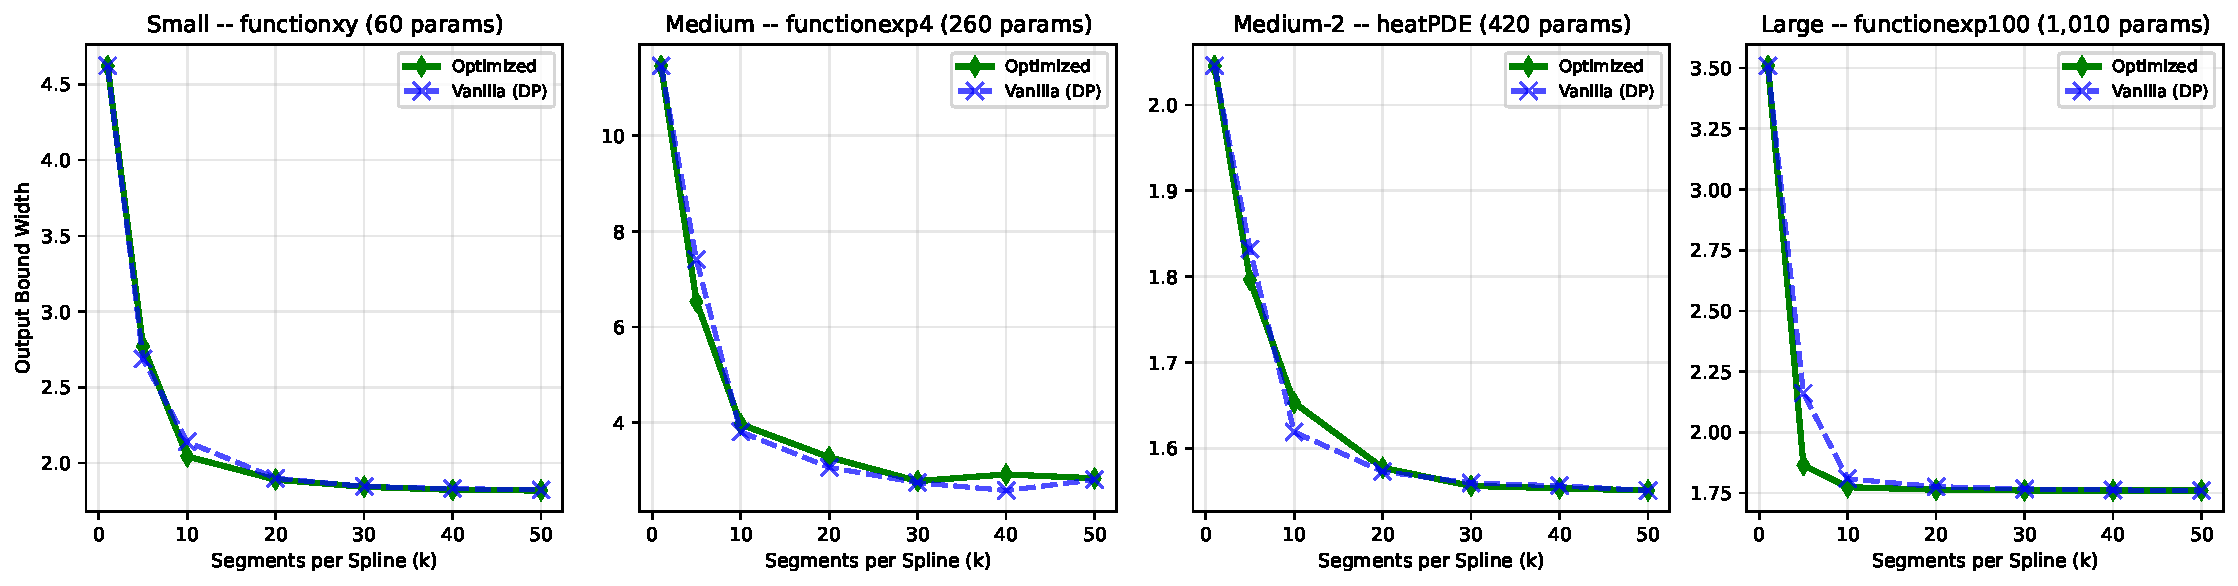
\includegraphics[width=1\linewidth, trim=5 5 5 5, clip]{images/plot_segments_vs_output_width.pdf}
    \caption{Output bound width as a function of per-spline segment budget $k$. \emph{Optimized} allocates the equivalent global budget $B = k \cdot |\mathcal{S}|$ via the ILP; \emph{Vanilla} assigns $k$ segments uniformly to every spline. At $k=1$ both methods coincide. For larger $k$, optimized allocation yields systematically tighter bounds, with the advantage largest at small $k$ where the ILP can most effectively concentrate segments on high-sensitivity splines, and narrowing as both methods saturate the underlying function. \{Small: [2, 2, 1] KAN; Medium: [4, 4, 2, 1] KAN; Medium-2: [2, 10, 2, 1] KAN; Large: [100, 1, 1] KAN; (x params): x trainable parameters per KAN\}}\label{fig:seg_width}
\end{figure*}

\section{More KAN benchmarks}\label{app:more-benchmarks}

We evaluate on five additional tasks from the original KAN paper~\cite{Liu+Others/2025/KAN}, chosen to stress the abstraction framework across a broader range of functional forms than the four main benchmarks. The tasks include a highly oscillatory function (Bessel), functions with rapidly varying curvature near the boundary of their domain (incomplete elliptic integrals), an associated Legendre polynomial evaluated via a wide single-hidden-layer network, and a bivariate special function (spherical harmonics). Together these benchmarks test whether the knapsack allocator's Lipschitz-weighted sensitivity reasoning transfers to functions whose curvature profiles differ substantially from the smooth exponentials and heat-equation solutions of the main evaluation. The five tasks are:

\begin{enumerate}
    \item \emph{Small}: \texttt{funcbessel}: $f(x) = \mathcal{J}_0(20 x)$ (1 input; 20 parameters; [1, 1] KAN). A highly oscillatory Bessel function of the first kind; the factor of $20$ compresses many oscillations into the unit interval, producing large, rapidly alternating curvature that challenges uniform PWA allocation.
    \item \emph{Small}: \texttt{funcellipeinc}: $f(x_1, x_2) = E(x_1\,|\,x_2)$, where $E(\phi\,|\,m)=\int_{0}^{\phi}\sqrt{1-m\sin^2\vartheta}\,d\vartheta$ (2 inputs; 70 parameters; [2, 2, 1, 1] KAN). An incomplete elliptic integral of the second kind; the integrand exhibits rapidly varying curvature as $m \to 1$, creating localized high-error regions where adaptive segment concentration is most beneficial.
    \item \emph{Medium}: \texttt{funcellipkinc}: $f(x_1, x_2) = K(x_1\,|\,x_2)$, where $K(\phi\,|\,m)=\int_{0}^{\phi}\frac{d\vartheta}{\sqrt{1-m\sin^2\vartheta}}$ (2 inputs; 70 parameters; [2, 2, 1, 1] KAN). An incomplete elliptic integral of the first kind; the denominator approaches zero more aggressively than in \texttt{funcellipeinc}, making this a harder approximation target with stronger curvature gradients.
    \item \emph{Small}: \texttt{funclegendre}: $f(x) = P_{\nu}^{m}(x)$, where $P_{\nu}^{m}(x) = (1-x^2)^{m/2}\,\frac{d^m}{dx^m}P_{\nu}(x)$ for integer $m\ge 0$ (1 input; 70 parameters; [1, 100, 1] KAN). The [1, 100, 1] architecture places 100 parallel splines in the single hidden layer, each receiving the same scalar input. Unlike the \emph{Large} benchmark, these splines approximate different nonlinear functions (different rows of the associated Legendre matrix), so their Lipschitz constants vary --- giving the knapsack allocator meaningful differentiation signal despite the wide single-layer structure.
    \item \emph{Small}: \texttt{funcsphharm}: $f(x_1, x_2) = \Re\{Y_{n}^{m}(x_1,x_2)\}$, where $Y_{n}^{m}(\theta,\phi)=\sqrt{\frac{2n+1}{4\pi}\frac{(n-m)!}{(n+m)!}}\,P_{n}^{m}(\cos\phi)\,e^{im\theta}$ (2 inputs; 140 parameters; [2, 3, 2, 1] KAN). The real part of a spherical harmonic; the function is smooth globally but exhibits oscillatory angular variation whose sensitivity profile differs across the two input dimensions, providing a bivariate test of cross-path sensitivity estimation.
\end{enumerate}

Figures~\ref{fig:input_width_small}, \ref{fig:seg_width_small}, and~\ref{fig:timing_small} report the input-width tightness, segment-budget tightness, and end-to-end timing results for these benchmarks respectively, mirroring the structure of Figures~\ref{fig:iw_width}, \ref{fig:seg_width}, and~\ref{fig:timing} in the main paper. The trends are consistent: \emph{Optimized} achieves tighter bounds across all input widths and segment budgets, with the largest gains at small perturbation radii and low segment budgets. The oscillatory and rapidly varying benchmarks (Bessel, elliptic integrals) tend to show relatively larger allocation gains, consistent with the expectation that high-curvature splines benefit most from targeted segment concentration.

\begin{figure*}[ht!]
    \centering
    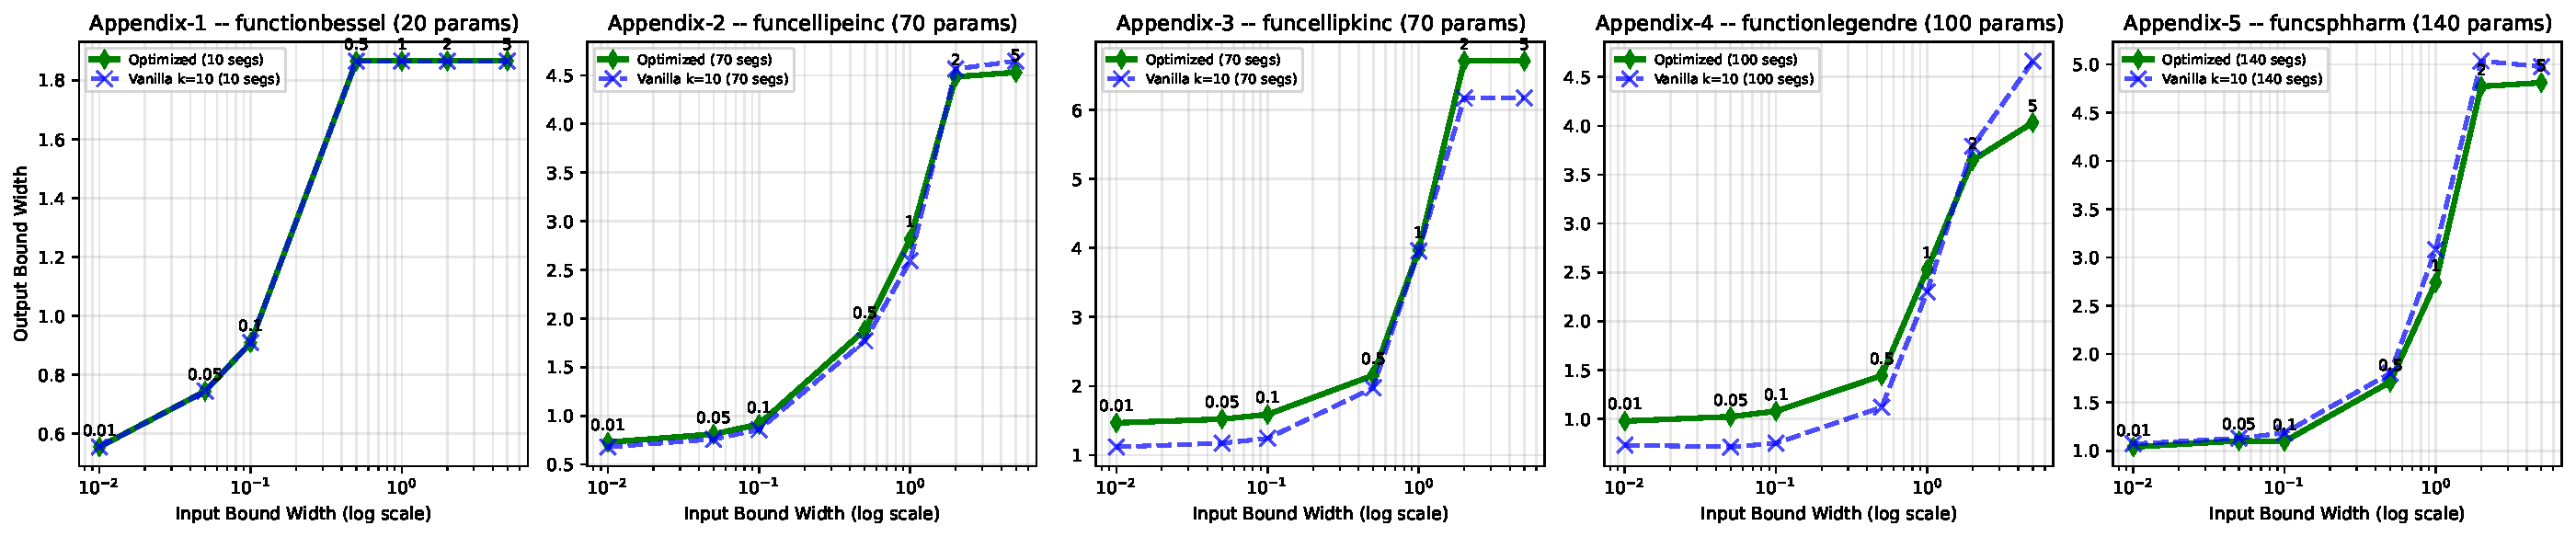
\includegraphics[width=1\linewidth, trim=5 5 5 5, clip]{images/plot_input_vs_output_width_small.pdf}
    \caption{Output bound width as a function of input perturbation radius $r$ for the additional benchmarks. The advantage of \emph{Optimized} over \emph{Vanilla} is most pronounced at small $r$, where tight bounds are operationally most valuable for robustness certification and the ILP allocator has the most leverage in concentrating segments along high-sensitivity spline paths.}\label{fig:input_width_small}
\end{figure*}

\begin{figure*}[ht!]
    \centering
    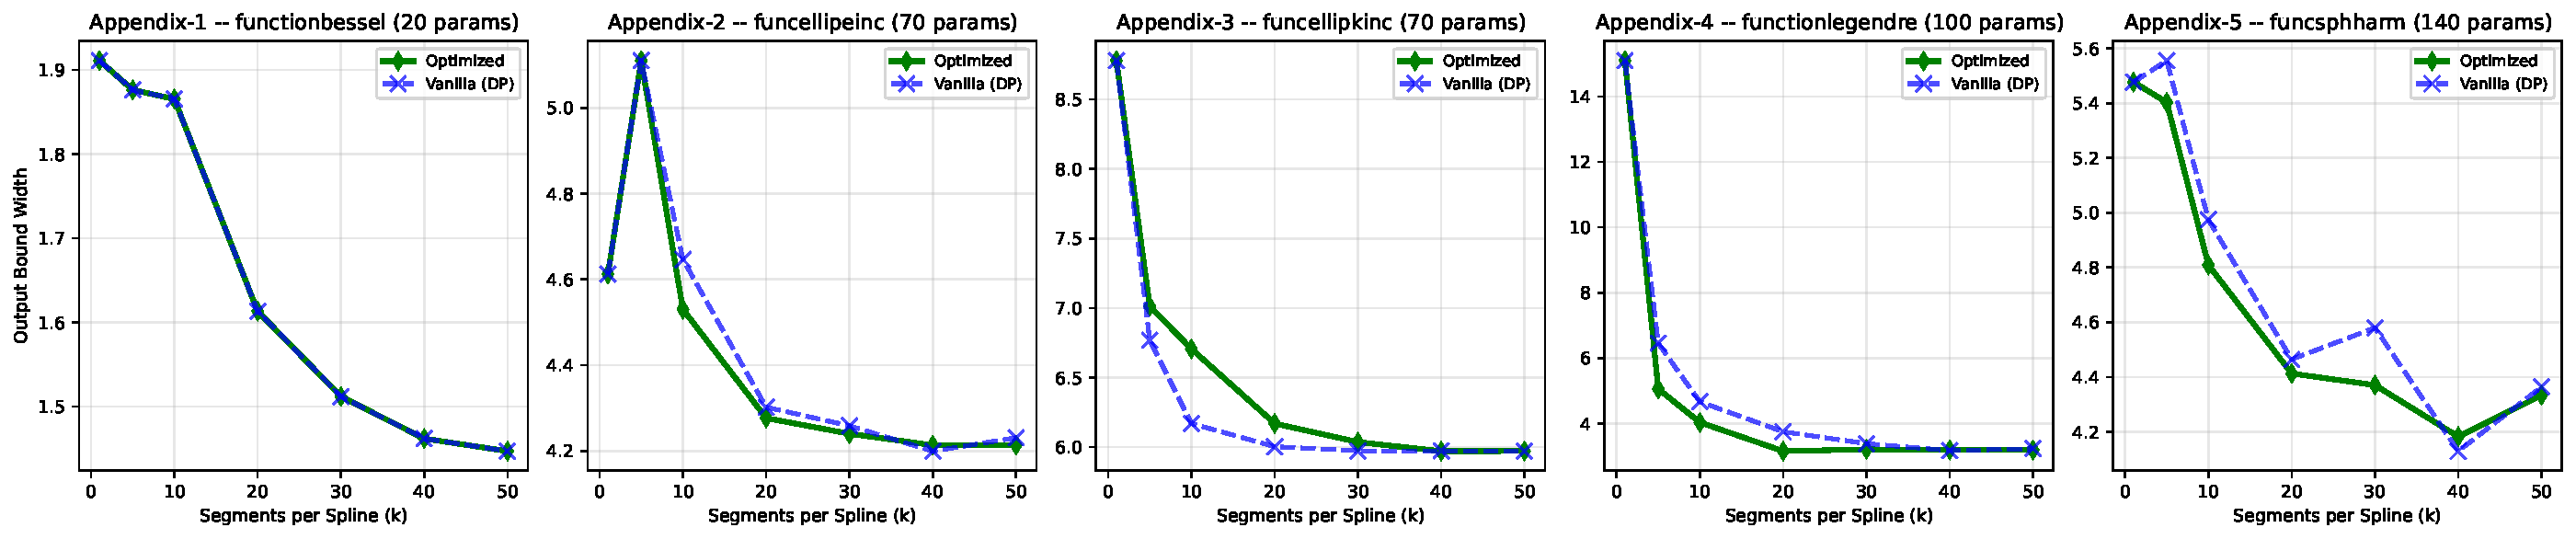
\includegraphics[width=1\linewidth, trim=5 5 5 5, clip]{images/plot_segments_vs_output_width_small.pdf}
    \caption{Output bound width as a function of segment budget $k$ for the additional benchmarks. \emph{Optimized} consistently achieves tighter bounds than \emph{Vanilla} at every budget level; the gain is largest at low $k$ where the ILP can most effectively concentrate segments on high-sensitivity splines, and narrows as both methods saturate the underlying function.}\label{fig:seg_width_small}
\end{figure*}

\begin{figure*}[ht!]
    \centering
    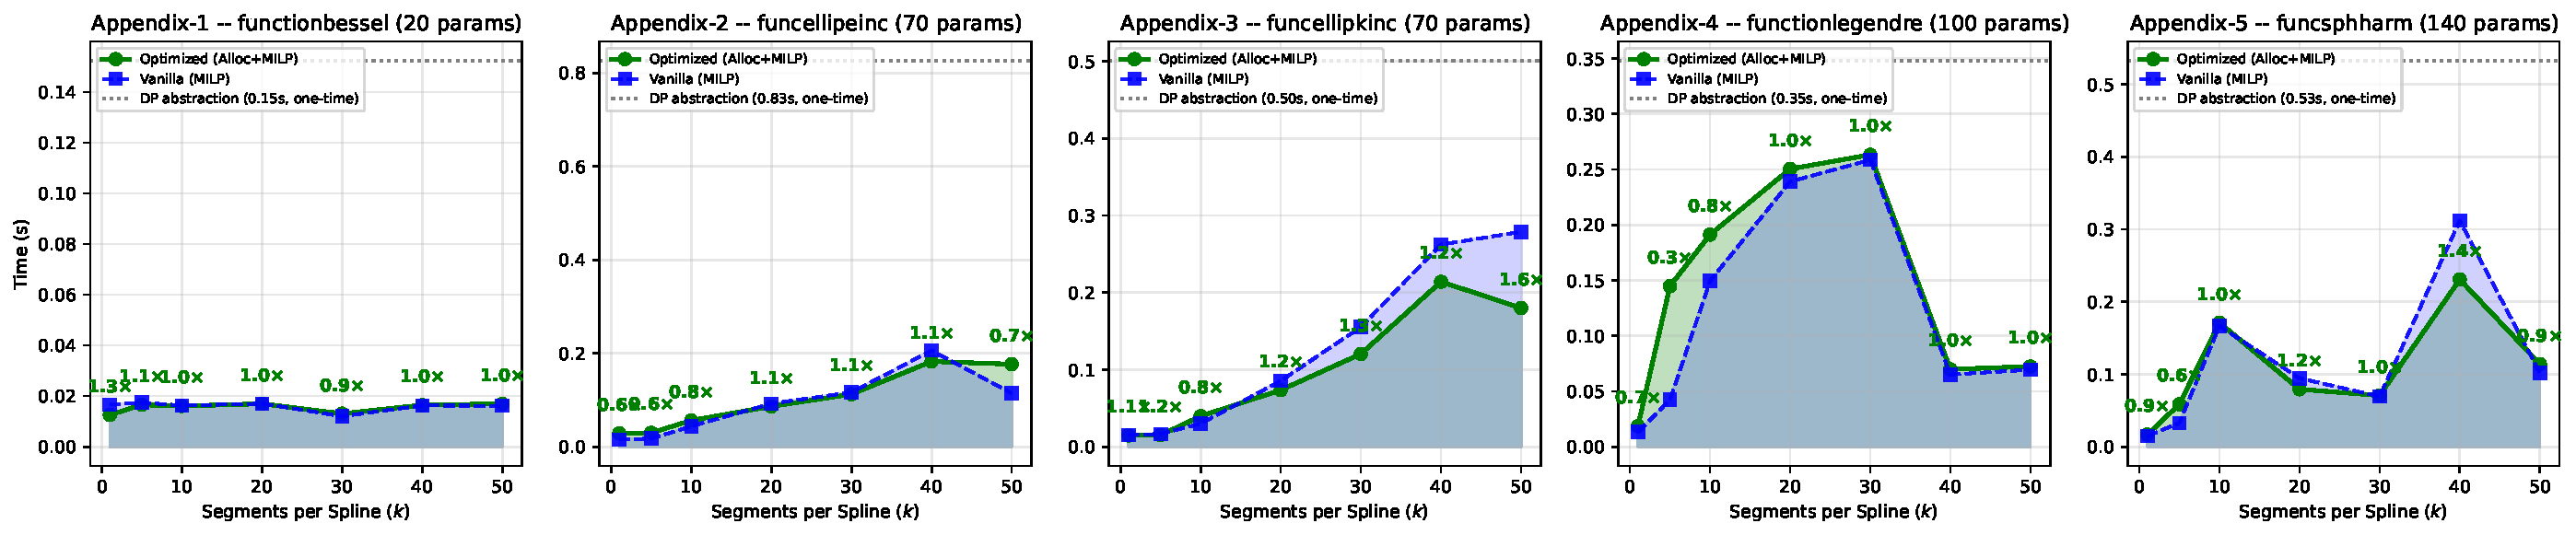
\includegraphics[width=1\linewidth, trim=5 5 5 5, clip]{images/plot_timing_summary_small.pdf}
    \caption{End-to-end runtime as a function of $k$ for the additional benchmarks. Optimized's per-query cost is the sum of the one-time DP abstraction (dotted line) and the downstream MILP (green); Vanilla incurs only the MILP cost (dashed). The multipliers on the green curve show the MILP-stage speedup, the relevant quantity when the abstraction is amortized across multiple verification queries on the same network.}\label{fig:timing_small}
\end{figure*}